\documentclass[10pt, a4paper]{article}

\usepackage[utf8]{inputenc}
\usepackage{helvet}
\renewcommand{\familydefault}{\sfdefault}
\usepackage[margin=0cm]{geometry}
\usepackage{xcolor}
\usepackage{tikz}
\usepackage{enumitem}
\usepackage{hyperref}
\usepackage{fontawesome5}
\usepackage{graphicx}

% Paleta de colores
\definecolor{headerbg}{HTML}{161E2E}     
\definecolor{sidebarbg}{HTML}{F8FAFC}    
\definecolor{accentblue}{HTML}{0284C7}   
\definecolor{darktext}{HTML}{1E293B}     
\definecolor{lightgray}{HTML}{64748B}    
\definecolor{timelinegray}{HTML}{CBD5E1} 
\definecolor{orcidgreen}{HTML}{A6CE39}   
\definecolor{white}{RGB}{255,255,255}

% Icono ORCID
\newcommand{\orcidicon}{%
    
\begin{tikzpicture}[baseline=-0.5ex]
        \fill[orcidgreen] (0,0) circle (3.8pt);
        \node[text=white, font=\fontsize{4pt}{4pt}\selectfont\bfseries] at (0,0) {iD};
    \end{tikzpicture}%
}

\hypersetup{
    colorlinks=true,
    urlcolor=accentblue,
    linkcolor=accentblue
}

\pagestyle{empty}
\setlength{\parindent}{0pt}

% Comandos visuales
\newcommand{\maintitle}[1]{%
    \vspace{3pt}%
    {\bfseries\fontsize{8.8pt}{10.5pt}\selectfont\color{darktext}\uppercase{#1}}\\[-3pt]%
    {\color{darktext}\rule{\linewidth}{1pt}}\par\vspace{2.5pt}%
}

\newcommand{\sidebadge}[1]{%
    \vspace{4pt}%
    \begin{tikzpicture}
        \node[fill=accentblue, text=white, font=\footnotesize\bfseries, inner sep=2.5pt, rounded corners=2pt] {#1};
    \end{tikzpicture}\par\vspace{2pt}%
}

\newcommand{\timelineentry}[3]{%
    \noindent
    \begin{tikzpicture}[baseline=(entrycontent.north)]
        \node[inner sep=0pt, outer sep=0pt, text width=12.2cm, align=left] (entrycontent) {
            {\fontsize{8.6pt}{10.5pt}\selectfont\textbf{\color{darktext} #1}} \hfill {\scriptsize\color{lightgray} #2}\\[1.5pt]
            #3
        };
        \draw[accentblue, line width=1.3pt] ([xshift=-7pt, yshift=-3.5pt]entrycontent.north west) -- ([xshift=-7pt, yshift=2pt]entrycontent.south west);
        \fill[accentblue] ([xshift=-7pt, yshift=-3.5pt]entrycontent.north west) circle (2.4pt);
    \end{tikzpicture}\par\vspace{2pt}
}

\begin{document}

% BANNER
\begin{tikzpicture}[remember picture, overlay]
    \fill[headerbg] (current page.north west) rectangle ([yshift=-3.4cm]current page.north east);
    \fill[sidebarbg] ([yshift=-3.4cm]current page.north west) rectangle ([xshift=6.7cm]current page.south west);
    \draw[timelinegray, line width=0.6pt] ([xshift=6.7cm, yshift=-3.4cm]current page.north west) -- ([xshift=6.7cm]current page.south west);

    \node[anchor=center, text width=\paperwidth, align=center] at ([yshift=-1.7cm]current page.north) {
        {\fontsize{20pt}{22pt}\selectfont\textbf{\color{white} ARTURO OLIVARES MARTOS}}\\[4pt]
        {\fontsize{9pt}{11pt}\selectfont\textbf{\color{accentblue!40} COMPUTER SCIENCE \& MATHEMATICS \enspace\textbar\enspace AI \& DATA SCIENCE}}\\[6pt]
        {\fontsize{7.5pt}{9.5pt}\selectfont\color{white!90}
        {\color{accentblue!40}\faMapMarker*} Granada, Spain \enspace\textbullet\enspace
        {\color{accentblue!40}\faEnvelope} \href{mailto:2004.olivares@gmail.com}{\color{white}2004.olivares@gmail.com} \enspace\textbullet\enspace
        \orcidicon \ \href{https://orcid.org/0009-0000-9415-7268}{\color{white!90}0009-0000-9415-7268} \enspace\textbullet\enspace
        {\color{accentblue!40}\faLinkedin} \href{https://linkedin.com/in/arturo-olivares-martos-4ba54b40a}{\color{white}arturo-olivares-martos} \enspace\textbullet\enspace
        {\color{accentblue!40}\faGithub} \href{https://github.com/arturo-olvrs}{\color{white}arturo-olvrs}
        }
    };
\end{tikzpicture}

\vspace*{3.65cm}

\begin{minipage}[t]{5.8cm}
    \vspace{0pt}\hspace{0.4cm}%
    \begin{minipage}[t]{5.2cm}
        \begin{center}
            \begin{tikzpicture}
                \begin{scope}
                    \clip (0,0) circle (1.3cm);
                    \node at (0,0) {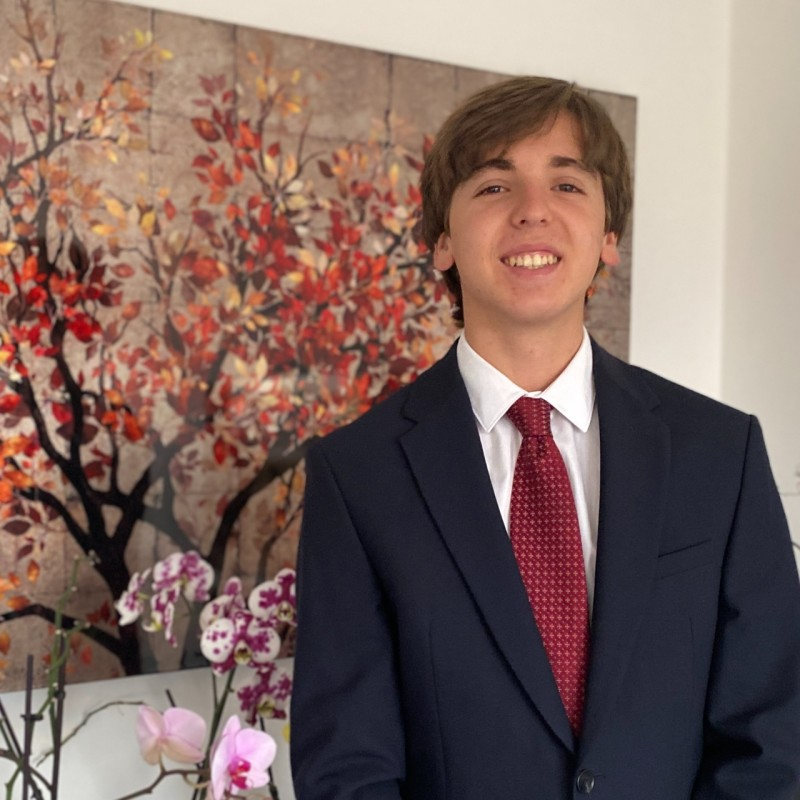
\includegraphics[width=2.6cm, height=2.6cm, keepaspectratio=false]{avatar_temp.jpg}};
                \end{scope}
                \draw[accentblue, line width=2.5pt] (0,0) circle (1.3cm);
            \end{tikzpicture}
        \end{center}
        \vspace{-6pt}

        \sidebadge{ABOUT ME}
        {\fontsize{6.8pt}{8.6pt}\selectfont\color{darktext}
        High-achieving student at UGR with international Erasmus exchange experience in Germany. Specialized at the intersection of rigorous mathematical modeling, advanced algorithms, and AI/MLOps engineering. Proven track record in scientific research, community leadership, and complex problem-solving.}\par

        \sidebadge{TECHNICAL SKILLS}
        {\fontsize{6.8pt}{8.8pt}\selectfont
        \textbf{\color{darktext} Languages \& Frameworks:}\\
        {\color{lightgray} Python, C++, TensorFlow, Scikit-Learn}\\[3pt]
        \textbf{\color{darktext} Modeling \& Mathematics:}\\
        {\color{lightgray} Optimization, Stochastic Models, Simulation, Advanced Algorithms}\\[3pt]
        \textbf{\color{darktext} Data Science \& Tools:}\\
        {\color{lightgray} Jupyter, Pandas, NumPy, Data Analysis}\\[3pt]
        \textbf{\color{darktext} Infrastructure \& DevOps:}\\
        {\color{lightgray} Git, GitHub, CI/CD, Docker, Google Cloud (GCP / MLOps)}
        }\par

        \sidebadge{LANGUAGES}
        {\scriptsize\textbf{\color{darktext} English:}} {\scriptsize\color{lightgray} C2 Proficiency (Cambridge)}\\[1.5pt]
        {\scriptsize\textbf{\color{darktext} German:}} {\scriptsize\color{lightgray} C1 (Goethe-Zertifikat)}\\[1.5pt]
        {\scriptsize\textbf{\color{darktext} French:}} {\scriptsize\color{lightgray} B2 (DELF International)}\\[1.5pt]
        {\scriptsize\textbf{\color{darktext} Spanish:}} {\scriptsize\color{lightgray} Native}

        \sidebadge{STUDY ABROAD \& IMMERSION}
        {\fontsize{6.6pt}{8.2pt}\selectfont
        \textbf{\color{darktext} Immersion in Berlin (Germany)}\\
        {\color{lightgray} GLS German Language School · Level B2.2 (2024)}\\[2.5pt]
        \textbf{\color{darktext} Immersion in Exmouth (UK)}\\
        {\color{lightgray} Hello! Exmouth · Level B2+ (2019)}\\[2.5pt]
        \textbf{\color{darktext} Immersion in Munich (Germany)}\\
        {\color{lightgray} Landheim Ammersee · Summer School · Level B1 (2019)}\\[2.5pt]
        \textbf{\color{darktext} Young Professionals in Oxford (UK)}\\
        {\color{lightgray} d'Overbroeck's · Engineering Course (2018)}
        }\par

        \sidebadge{CERTIFICATIONS}
        {\fontsize{6.6pt}{8.2pt}\selectfont
        \textbf{\color{darktext} MLOps for Generative AI}\\
        {\color{lightgray} Google Cloud Skills Boost · 2026}\\[2pt]
        \textbf{\color{darktext} Logic and Set Theory}\\
        {\color{lightgray} UGR Micro-credential · 2025}\\[2pt]
        \textbf{\color{darktext} Youth Activity Leader \& Leisure Monitor}\\
        {\color{lightgray} Regional Government of Andalusia · 2022}
        }\par
    \end{minipage}
\end{minipage}%
\hfill
\begin{minipage}[t]{13.1cm}
    \vspace{0pt}

    \maintitle{EDUCATION \& ACADEMIC RECORD}

    \timelineentry{B.Sc. in Computer Science and B.Sc. in Mathematics (Double Degree)}{2022 -- 2027}{%
        {\footnotesize\textbf{\color{accentblue} University of Granada (UGR)}} \hfill {\scriptsize\color{lightgray} Granada, Spain}\\[1.5pt]
        \begin{itemize}[leftmargin=*, nosep, topsep=1pt, itemsep=1.5pt]
            \item \textbf{GPA: 9.2 / 10}.
            \item Specialization in AI, Data Science, and Mathematical Optimization.
        \end{itemize}
    }

    \timelineentry{Erasmus+ Exchange \textbar\ Computer Science \& Data Science}{2025 -- 2026}{%
        {\footnotesize\textbf{\color{accentblue} University of Duisburg-Essen}} \hfill {\scriptsize\color{lightgray} Duisburg, Germany}\\[1.5pt]
        \begin{itemize}[leftmargin=*, nosep, topsep=1pt, itemsep=1.5pt]
            \item International exchange; master-level coursework in modeling and AI.
        \end{itemize}
    }

    \timelineentry{High School Diploma in Science and Technology}{2020 -- 2022}{%
        {\footnotesize\textbf{\color{accentblue} Marist Brothers School (HH. Maristas)}} \hfill {\scriptsize\color{lightgray} Granada, Spain}\\[1.5pt]
        \begin{itemize}[leftmargin=*, nosep, topsep=1pt, itemsep=1.5pt]
            \item \textbf{2nd highest University Entrance Exam (PEvAU) score} in the province of Granada (\textbf{13.975 / 14.000}).
        \end{itemize}
    }

    \timelineentry{Dual American High School Diploma}{2019 -- 2022}{%
        {\footnotesize\textbf{\color{accentblue} Academica International Studies}} \hfill {\scriptsize\color{lightgray} USA / Online}
    }

    \vspace{3pt}

    \maintitle{LEADERSHIP \& DIGITAL COMMUNITY}

    \timelineentry{Founder \& Lead Coordinator}{Sept. 2022 -- Present}{%
        {\footnotesize\textbf{\color{accentblue} Los Del DGIIM (UGR Community)}} \hfill {\scriptsize\color{lightgray} Granada, Spain}\\[1.5pt]
        \begin{itemize}[leftmargin=*, nosep, topsep=1pt, itemsep=1.5pt]
            \item Founded the official community network for the Double Degree; managing channels with hundreds of students.
            \item Maintain GitHub repositories featuring codebases, study resources, and software architectures with widespread adoption.
        \end{itemize}
    }

    \maintitle{RESEARCH, CONFERENCES \& OUTREACH}

    \begin{itemize}[leftmargin=*, nosep, topsep=1pt, itemsep=2pt]
        \item \href{https://doi.org/10.5334/jors.771}{\textbf{\color{darktext}\footnotesize Making Soundscape Assessment Accessible: The SoundGraphy Tool \faExternalLink*}} \hfill {\scriptsize\color{lightgray} Sept. 2026}\\
        {\scriptsize\textit{Journal of Open Research Software (JORS) -- Ubiquity Press (Vol. 14: 63)}}\\
        {\scriptsize First author and software developer for soundscape analysis and visualization (ISO 12913 \& SSM).}
        \item \href{https://dl.gi.de/items/4b863f76-35d4-4ec3-a18b-427b56539919}{\textbf{\color{darktext}\footnotesize Monitoring and Understanding Notebook-Based Learning with Jupyter \faExternalLink*}} \hfill {\scriptsize\color{lightgray} Duisburg · Sept. 2026}\\
        {\scriptsize\textit{Mensch und Computer (MuC 2026) -- German Informatics Society (GI)}}\\
        {\scriptsize Co-authored research on learning analytics, student monitoring, and interactive dashboards.}
        \item \textbf{\color{darktext}\footnotesize University Delegate at AIvolution Conference} \hfill {\scriptsize\color{lightgray} Brussels · 2023}\\
        {\scriptsize\textit{European Parliament (Renew Europe)}: Selected to debate alongside international experts on the socioeconomic impact of AI, digital rights, cybersecurity, and technological regulation.}
        \item \href{https://revistasuma.es/wp-content/uploads/suma/Suma104/S104w_039-052.pdf}{\textbf{\color{darktext}\footnotesize Mathematical Modeling, Vaccination, and Python \faExternalLink*}} \hfill {\scriptsize\color{lightgray} Granada · Aug. 2022}\\
        {\scriptsize\textit{SUMA+ Scientific Journal (No. 104, pp. 39-52)}: Supply chain and logistical optimization for COVID-19 distribution.}
        \item \textbf{\color{darktext}\footnotesize Guest Speaker in Computational Modeling} \hfill {\scriptsize\color{lightgray} CEFIRE Valencia · Feb. 2021}\\
        {\scriptsize Delivered technical training for educators on real-world applications of mathematical modeling and simulation.}
    \end{itemize}

    \maintitle{HONORS \& AWARDS}

    \begin{itemize}[leftmargin=*, nosep, topsep=1pt, itemsep=1.5pt]
        \item \textbf{\color{darktext}\footnotesize Two-time National Champion \& Global Honorable Mention -- IMMC} \hfill {\scriptsize\color{lightgray} 2020, 2021}\\
        {\scriptsize 1st place in Spain (two consecutive years) and Global Honorable Mention at the \textit{International Mathematical Modeling Challenge (IMMC)} for multivariate optimization.}
        \item \textbf{\color{darktext}\footnotesize 1st National Chemistry Prize (\#STEM\_for\_Teens)} \hfill {\scriptsize\color{lightgray} Apr. 2019}\\
        {\scriptsize National recognition awarded by Google, the Spanish Royal Academy of Sciences, and Junior Achievement.}
        \item \textbf{\color{darktext}\footnotesize Runner-up / Honorable Mention, XXXIV THALES Mathematical Olympiad} \hfill {\scriptsize\color{lightgray} Apr. 2018}
    \end{itemize}

    \maintitle{SOCIAL COMMITMENT \& VOLUNTEERING}

    \begin{itemize}[leftmargin=*, nosep, topsep=1pt, itemsep=1.5pt]
        \item \textbf{\footnotesize Student Volunteer:} MuC 2026 Conference (German Informatics Society). \hfill {\scriptsize\color{lightgray} Aug. 2026}
        \item \textbf{\footnotesize Youth \& Leisure Activity Leader:} Maristas Mediterranean Province. \hfill {\scriptsize\color{lightgray} 2021 -- Present}
        \item \textbf{\footnotesize Community Outreach:} Daughters of Charity Soup Kitchen \& Córdoba Autism Association.
    \end{itemize}

\end{minipage}
\hspace{0.4cm}

\end{document}